\documentclass[compress,12pt]{beamer}

% \usepackage{amsmath,amsthm,amssymb,amsfonts,layout,verbatim}

\usepackage{url}

% \usepackage[
% bookmarks=true,
% colorlinks=true,
% pdftex,
% linkcolor=black,
% filecolor=blue,
% pagecolor=blue,
% urlcolor=blue]
% {hyperref}

% Useful macros to keep around
\newcommand{\bv}[1]{{\boldsymbol{#1}}}
\newcommand{\D} [2]{\frac{\partial #1}{\partial #2}}
\newcommand{\textD}[2]{\tfrac{\partial #1}{\partial #2}} % forces a text fraction (smaller)
%\newcommand{\KT}{\mbox{$\kappa^{*}$}}
%%\newcommand{\bv}[1]{{\boldsymbol{#1}}}

\setbeamercovered{invisible}


% \hyperbaseurl{/home/peterson/work/FE_Rodeo_2006/}

\title{A Stabilized $h$-Adaptive Continuation Method for
  Double-Diffusive Convection in Porous Media}
\author{J.~W.~Peterson\inst{1} \and B.~T.~Murray\inst{2} \and G.~F.~Carey\inst{3}}
\institute{
\inst{1}Dept. of Aerospace Engineering \& Eng.~Mech., UT-Austin
\and
\inst{2}Dept. of Mech. Eng., SUNY Binghamton
\and
\inst{3}Inst.~for Computational Engineering \& Sciences (ICES), UT-Austin
}

\date{March 3-4, 2006}


% \MyLogo{FE Rodeo 2006 -- College Station, TX}
% \rightheader{\includegraphics[height=.7in]{figures/word3}}
% \leftheader{\includegraphics[height=.7in]{figures/utlogo}}

\begin{document}

\begin{frame}
  \titlepage
\end{frame}

% TODO: Use sections and then uncomment this line
% \section*{Outline}% Make it easy to jump to this page in the PDF

% use outline_currentsection.tex to highlight the current section

% Auto-generate the TOC slide(s)
\begin{frame}
  %\tableofcontents[currentsection]
  \tableofcontents
\end{frame}




%%%%%%%%%%%%%%%%%%%%%%%%%%%%%%%%%%%%%%%%%%%%%%%%%%%%%%%%%%%%%%%%%%%%%%%%%%%%%%%
\begin{frame}{Introduction}
  \begin{itemize}
    \item ``Double-diffusive'' effects occur whenever there are
      opposing gradients of two diffusing components, each of which affects
      the local density of a fluid.

    \item In thermo-solutal convection, the competing components are solute concentration
      and heat (e.g. a differentially heated layer of sand saturated
      with brine)

    \item In this talk, we consider an extremely simple double-diffusive
      system, and develop a stabilized adaptive finite element method for computing accurate
      solutions under different parametric regimes.
      
  \end{itemize}
\end{frame}




%%%%%%%%%%%%%%%%%%%%%%%%%%%%%%%%%%%%%%%%%%%%%%%%%%%%%%%%%%%%%%%%%%%%%%%%%%%%%%%
\begin{frame}{Governing Equations}
  \begin{itemize}
    \item The equations model slow flow through saturated porous media with
      buoyancy effects (see e.g.\ Nield \& Bejan, 1992)
  \end{itemize}
  \begin{equation}
    \nonumber
    \label{eqn:div-free}
    \nabla \cdot \bv{u} = 0 
  \end{equation}
    %
  \begin{equation}
    \nonumber
    \label{eqn:mom}
    \frac{\rho_0}{\epsilon} \D{\bv{u}}{t} = - \nabla p + \rho \bv{g} - \frac{\mu}{K} \bv{u} 
  \end{equation}
    %
  \begin{equation}
    \nonumber
    \label{eqn:T}
    \sigma \D{T}{t} +  \bv{u} \cdot \nabla T = \kappa_T \Delta T 
  \end{equation}
    %
  \begin{equation}
    \nonumber
    \label{eqn:S}
    \epsilon \D{S}{t} + \bv{u} \cdot \nabla S = \kappa_S \Delta S
  \end{equation}

    
  \begin{equation}
    \nonumber
    \rho = \rho_0 [ 1 - \alpha ( T - T_{0} ) + \beta ( S - S_{0} ) ]
  \end{equation}

% $\bv{u}$ is the filtration or Darcy velocity
% $T$, $S$, and $\rho$ are temperature, solute concentration, and density
% $\epsilon$ is the porosity of the porous medium
% $K$ is the permeability,
% $\mu$ is the absolute viscosity
% $M = ( \rho c)_f / ( \rho c)_m$) the heat capacity ratio; *** sigma = 1/M ***
% \kappa_S is the _effective_ solute diffusivity
% \kappa_T is the _effective_ temp diffusivity
% $\alpha$ is the thermal expansion coefficient
% $\beta$ is the solute expansion coefficient. 

\end{frame}







%%%%%%%%%%%%%%%%%%%%%%%%%%%%%%%%%%%%%%%%%%%%%%%%%%%%%%%%%%%%%%%%%%%%%%%%%%%%%%%
\begin{frame}{Problem Description}
%\begin{itemize}
%%   \item The goal is to develop a stabilized adaptive finite element method
%%     to investigate the stability characteristics of doubly-diffusive systems.

%%   \item The region of the parameter space of interest in these calculations is
%%     quite large, with solutions exhibiting oscillatory onset of convection and
%%     thin layers with high heat and solute transfer rates.

%%   \item Efficient calculation of these solutions (especially in 3D) is necessary
%%     to draw fundamental conclusions about the system.
%\end{itemize}
  \centerline{\includegraphics[width=.55\textwidth]{figures/setup3d}}
\begin{itemize}
  \item $\bv{u} \cdot \hat{n}=0 \in \Gamma = \Gamma_{\text{top}}
    \cup \Gamma_{\text{side}} \cup \Gamma_{\text{bot}}$
    \item Solute and temperature values fixed on $\Gamma_{\text{top}}$ and $\Gamma_{\text{bot}}$
    \item No solute or temperature flux from $\Gamma_{\text{side}}$
\end{itemize}

\end{frame}





%%%%%%%%%%%%%%%%%%%%%%%%%%%%%%%%%%%%%%%%%%%%%%%%%%%%%%%%%%%%%%%%%%%%%%%%%%%%%%%
\begin{frame}{Non-Dim Eqns.}
  \begin{itemize}
    \item After manipulation, the standard non-dimensional equations are
  \end{itemize}

  \begin{eqnarray}
    \nonumber
    \label{eqn:mom-nondim}
    \nabla \cdot \bv{b} - \Delta p &=& 0 \\
  %
    \nonumber
    \label{eqn:T-nondim}
    \D{T}{t} +  (\bv{b}- \nabla p) \cdot \nabla T  - \Delta T &=& 0 \\
  %
    \nonumber
    \label{eqn:S-nondim}
    \frac{\epsilon}{\sigma} \D{S}{t} + (\bv{b} -
    \nabla p) \cdot \nabla S  - \kappa \Delta S &=&  0
  \end{eqnarray}
  where
  \begin{equation}
    \label{eqn:buoyant_force}
    \bv{b}:=(\kappa R_S S - R_T T)\hat{e}_g
  \end{equation}

  \begin{equation}
    \label{eqn:kappa}
    \kappa = 1/Le := \kappa_S / \kappa_T \ll 1
  \end{equation}

\end{frame}



%%%%%%%%%%%%%%%%%%%%%%%%%%%%%%%%%%%%%%%%%%%%%%%%%%%%%%%%%%%%%%%%%%%%%%%%%%%%%%%
\begin{frame}{Rayleigh Numbers}
  \begin{itemize}
%    \tightlist
%%     \item The equations are non-dimensionalized with length scale $d$ (vertical depth),
%%       time scale $d^2 \sigma / \kappa_T$, velocity scale $\kappa_T / d$,
%%       temperature scale $\delta T$, and solutal scale $\delta S$.

    \item The thermal and solutal
      Rayleigh numbers are defined as
  \end{itemize}
      
      \begin{equation}
	\nonumber
	R_T = \frac{ g  K  d \alpha }{\nu \kappa_T} \delta T
      \end{equation}	%
      
      \begin{equation}
	\nonumber
	R_S = \frac{ g   K  d \beta}{\nu  \kappa_S}  \delta S
      \end{equation}	%

      \begin{itemize}
      \item Total solute flux is selected as the ``Quantity of Interest''.
      \end{itemize}
%%     \item A Poisson equation for the pressure is obtained by taking the divergence
%%       of Eqn.~\eqref{eqn:mom} and enforcing the $\nabla \cdot \bv{u}=0$ condition.

%%     \item Generally, $\kappa \ll 1$ since solute diffuses
%%       in the medium more slowly than heat.
      
    %\item $\epsilon / \sigma = \mathcal{O}(1)$, so the equations are not very ``stiff''
\end{frame}








%%%%%%%%%%%%%%%%%%%%%%%%%%%%%%%%%%%%%%%%%%%%%%%%%%%%%%%%%%%%%%%%%%%%%%%%%%%%%%%
\begin{frame}{Remarks}
  \begin{itemize}
    \item A steady, quiescent solution with $\hat{e}_g=-\hat{k}$, $0 \leq z \leq 1$ is given by
      \begin{eqnarray}
	\label{eqn:p-base}\nonumber
	p_0 &=& \phantom{\kappa}R_T\left[T_{\text{bot}}z + \tfrac{z^2}{2}(T_{\text{top}}-T_{\text{bot}})\right]-\\
	\nonumber
	&\phantom{=}& \kappa R_S \left[S_{\text{bot}}z + \tfrac{z^2}{2}(S_{\text{top}}-S_{\text{bot}})\right]\\
	\label{eqn:T-base}\nonumber
	T_0 &=& T_{\text{bot}} + z(T_{\text{top}}-T_{\text{bot}})  \\
	\label{eqn:S-base}\nonumber
	S_0 &=& S_{\text{bot}} + z(S_{\text{top}}-S_{\text{bot}}) 
      \end{eqnarray}

%%     \item Depending on the parameters, this base solution may be stable or unstable to
%%       finite size perturbations.
      
  \end{itemize}
  
  % \centerline{\includegraphics[height=1.5in]{figures/plumes}}

\end{frame}


% %%%%%%%%%%%%%%%%%%%%%%%%%%%%%%%%%%%%%%%%%%%%%%%%%%%%%%%%%%%%%%%%%%%%%%%%%%%%%%%
% \begin{frame}{Remarks (2)}
%   \begin{itemize}
% %%   \item The ``natural'' boundary condition for Eqn.~\eqref{eqn:mom-nondim}
% %%     \begin{equation}
% %%       (\bv{b} - \nabla p) \cdot \hat{n} = 0 \in \Gamma
% %%     \end{equation}
% %%     is equivalent to the no-penetration ($\bv{u} \cdot \hat{n}$ =0) condition
% %%     imposed on the domain.
%   \item An important quantity of interest will be the 
%     solutal Nusselt number
%       \begin{equation}
% 	\nonumber
% 	N_S := -\int_{\Gamma_{D}} \! (\nabla S \cdot \hat{n}) \;dx
%       \end{equation}
% %      This value will be used to compare solutions on different grids.
%   \end{itemize}
% \end{frame}




%%%%%%%%%%%%%%%%%%%%%%%%%%%%%%%%%%%%%%%%%%%%%%%%%%%%%%%%%%%%%%%%%%%%%%%%%%%%%%%
\begin{frame}{Numerical Method}

  \begin{itemize}
    \item Implicit time discretization (Crank-Nicolson), bilinear
      Lagrange elements, coupled solve for $p$, $T$, and $S$.

    \item A simple adaptive continuation algorithm in $\kappa$:
      \begin{enumerate}
	\item Start with moderate $\kappa$, evolve solution by timestepping from
	  quiescent initial state to steady convecting state.
	\item $h$-adapt mesh to new state.
	\item Decrease $\kappa$, use adapted mesh as new initial condition.
	\item Use steady state equations to converge solution at new $\kappa$.
	\item Return to step 2 until finished.
      \end{enumerate}

      %    \item One or two refinement steps per timestep

%%     \item Time-accurate $h$-adaptive refinement schemes are relatively
%%       expensive (this avoids that to some extent).
%%     \item The grid is not always ``optimal'' during the time evolution stage,
%%       but this is OK for reasonable steps in $\kappa$.
      
    \item Essentially allows accurate parameter space mappings but relies
      on the solution being stable on the initial coarse grid.
  \end{itemize}

\end{frame}



%%%%%%%%%%%%%%%%%%%%%%%%%%%%%%%%%%%%%%%%%%%%%%%%%%%%%%%%%%%%%%%%%%%%%%%%%%%%%%%
\begin{frame}{Numerical Method (cont.)}
  \begin{itemize}
  \item For small values of $\kappa$, the standard Galerkin method is unstable
    on coarse grids.
  \item Solutal Peclet number based on domain height $d=1$:
    \begin{equation}
      \nonumber
      \max_{\Omega} Pe_S = \max_{\Omega} \frac{|\bv{b}-\nabla p|}{\kappa}
      % = \mathcal{O}\left(10^2\right) - \mathcal{O}\left(10^3\right) 
    \end{equation}
    is $\mathcal{O}\left(10^2\right)$ --- $\mathcal{O}\left(10^3\right)$
    for the cases of interest here.

  \item An SUPG-type stabilized formulation (with nonlinear, scalar $\tau$)
    is applied to the solute equation only, the $p$ and $T$ equations are
    solved with standard Galerkin.
    
    %%     \item Hierarchical $h$-refinement with constrained hanging nodes, level-1 rule,
    %%       and maximum refinement level of 2 with respect to the coarse mesh
    %%       \centerline{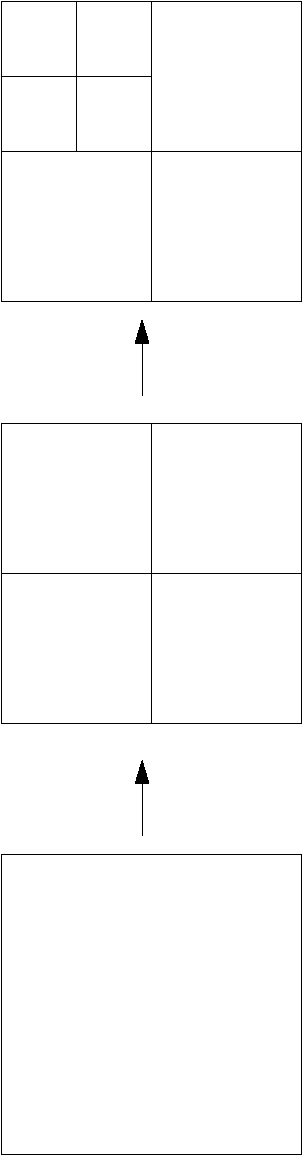
\includegraphics[height=.80\textwidth,angle=-90]{figures/refinement}}
    
    %%     \item Error indicator is the generic Kelly et.\ al indicator, jumps in the
    %%       inter-element solutal flux drive the refinement patterns
    
    %%     \item Refinement flagging scheme is based on assumed (log) normal distribution
    %%       of the element errors
    %%     \centerline{\includegraphics[angle=-90,width=.6\textwidth]{figures/ref_scheme}}
      
  \end{itemize}

\end{frame}


%%%%%%%%%%%%%%%%%%%%%%%%%%%%%%%%%%%%%%%%%%%%%%%%%%%%%%%%%%%%%%%%%%%%%%%%%%%%%%%
\begin{frame}{Linear Stability Theory}
  \begin{minipage}[h]{.45\textwidth}
    \begin{itemize}
    \item Linear stability diagram for the destabilizing thermal / stabilizing solute configuration
    \item The diffusivity ratio (in the figure $\tau \equiv \kappa$) affects the mechanism for onset of convection
    %\item We conduct a 2D numerical experiment to determine the effect that
    %  varying $\kappa$ has on the Nusselt number computations in the steady onset regime
    \end{itemize}
  \end{minipage}
  \hspace{.1in}
  \begin{minipage}[h]{.5\textwidth}
  \centerline{\includegraphics[height=.85\textheight]{figures/stability_diagram}}
  \end{minipage}
\end{frame}




%%%%%%%%%%%%%%%%%%%%%%%%%%%%%%%%%%%%%%%%%%%%%%%%%%%%%%%%%%%%%%%%%%%%%%%%%%%%%%%
\begin{frame}{Numerical Experiment}
  \begin{minipage}[h]{.45\textwidth}
    \begin{itemize}
    \item Parameter values in the steady onset regime were chosen
      \begin{eqnarray}
	\nonumber
	R_T=200 \\%,  \hspace{.25in}
	\nonumber
	R_S=160 \\%, \hspace{.25in}
	\nonumber
	\epsilon / \sigma = 1/3
      \end{eqnarray}
    \end{itemize}
  \end{minipage}
  %
  \begin{minipage}[h]{.45\textwidth}
    \begin{figure}
      \begin{center}
      \includegraphics[height=.35\textheight,angle=-90]{figures/initial_profile2}
      \caption{Initial profiles}
      \end{center}
    \end{figure}
  \end{minipage}

  \begin{itemize}
    \item The equations were solved using the continuation algorithm
      for 
      \begin{equation}
	\nonumber
	0.01 \leq \kappa \leq 0.1
      \end{equation}
      using both uniform and $h$-adaptive grids.
    % \item Maximum and steady state Nusselt numbers were recorded.

  \end{itemize}
\end{frame}




%%%%%%%%%%%%%%%%%%%%%%%%%%%%%%%%%%%%%%%%%%%%%%%%%%%%%%%%%%%%%%%%%%%%%%%%%%%%%%%
\begin{frame}{Numerical Experiment (cont.)}
  \only<1>
    {
      \begin{center}\begin{tabular}{cc} \\
	\includegraphics[width=.5\textwidth]{figures/s_80x80_kappa_0_10}&
	\includegraphics[width=.5\textwidth]{figures/s_adapt_kappa_0_10}\\
	Uniform &
	Adaptive
      \end{tabular}\end{center}
      \begin{itemize}
      \item Solute density contours for $\kappa=0.1$.
      \end{itemize}
    }

    \only<2>
    {
      \begin{center}\begin{tabular}{cc} \\
	\includegraphics[width=.5\textwidth]{figures/grid_80x80}&
	\includegraphics[width=.5\textwidth]{figures/grid_adapt_kappa_0_10}\\
	19,683 dofs &
	3825 dofs
      \end{tabular}\end{center}
    }

    \only<3>
    {
     \begin{center}\begin{tabular}{cc} \\
      \includegraphics[width=.5\textwidth]{figures/s_80x80_kappa_0_03}&
      \includegraphics[width=.5\textwidth]{figures/s_adapt_kappa_0_03}\\
      Uniform &
      Adaptive
     \end{tabular}\end{center}
     \begin{itemize}
       \item Solute density contours for $\kappa=0.03$.
     \end{itemize}
    }

    \only<4>
    {
      \begin{center}\begin{tabular}{cc} \\
	\includegraphics[width=.5\textwidth]{figures/grid_80x80}&
	\includegraphics[width=.5\textwidth]{figures/grid_adapt_kappa_0_03}\\
	19,683 dofs &
	32,787 dofs
      \end{tabular}\end{center}
    }
\end{frame}



%%%%%%%%%%%%%%%%%%%%%%%%%%%%%%%%%%%%%%%%%%%%%%%%%%%%%%%%%%%%%%%%%%%%%%%%%%%%%%%
\begin{frame}{Convergence}
  \begin{center}
    \includegraphics[viewport=124 40 670 550,width=.65\textwidth,clip=true]{figures/s_x_equal_0_point_5}
    \begin{itemize}
    \item Solute density $s(y)$ along the centerline $x=0.5$ for $\kappa=0.03$.
    \end{itemize}
  \end{center}      
\end{frame}



%%%%%%%%%%%%%%%%%%%%%%%%%%%%%%%%%%%%%%%%%%%%%%%%%%%%%%%%%%%%%%%%%%%%%%%%%%%%%%%
\begin{frame}{Convergence}
  \begin{center}
    \begin{tabular}{cc} \\
      \includegraphics[viewport=124 40 670 550,clip=true,width=.5\textwidth]{figures/s_x_equal_0_point_5_zoom_0}&
      \includegraphics[viewport=124 40 670 550,clip=true,width=.5\textwidth]{figures/s_x_equal_0_point_5_zoom_1}\\
      $s(y)$ near $y=0$ &
      $s(y)$ near $y=1$ 
    \end{tabular}
    \begin{itemize}
    \item Solute density $s(y)$ along the centerline $x=0.5$ for $\kappa=0.03$.
    \end{itemize}
  \end{center}    
\end{frame}


%%%%%%%%%%%%%%%%%%%%%%%%%%%%%%%%%%%%%%%%%%%%%%%%%%%%%%%%%%%%%%%%%%%%%%%%%%%%%%%
\begin{frame}{Convergence}
  \begin{center}
    \includegraphics[viewport=124 40 670 550,width=.65\textwidth,clip=true]{figures/s_x_equal_0_point_25}
    \begin{itemize}
    \item Solute density $s(y)$ along the quarter-line $x=0.25$ for $\kappa=0.03$.
    \end{itemize}
  \end{center}      
\end{frame}



%%%%%%%%%%%%%%%%%%%%%%%%%%%%%%%%%%%%%%%%%%%%%%%%%%%%%%%%%%%%%%%%%%%%%%%%%%%%%%%
\begin{frame}{Convergence}
  \begin{center}
    \begin{tabular}{cc} \\
      \includegraphics[viewport=124 40 670 550,clip=true,width=.5\textwidth]{figures/s_x_equal_0_point_25_zoom_0}&
      \includegraphics[viewport=124 40 670 550,clip=true,width=.5\textwidth]{figures/s_x_equal_0_point_25_zoom_1}\\
      $s(y)$ near $y=0$ &
      $s(y)$ near $y=1$ 
    \end{tabular}
    \begin{itemize}
    \item Solute density $s(y)$ along the quarter-line $x=0.25$ for $\kappa=0.03$.
    \end{itemize}
  \end{center}    
\end{frame}




%%%%%%%%%%%%%%%%%%%%%%%%%%%%%%%%%%%%%%%%%%%%%%%%%%%%%%%%%%%%%%%%%%%%%%%%%%%%%%%
\begin{frame}{Adaptive Solutions}
  \only<1>
  {
    \begin{center}
      \begin{tabular}{cc} \\
	\includegraphics[width=.5\textwidth]{figures/s_adapt_kappa_0_10}&
	\includegraphics[width=.5\textwidth]{figures/grid_adapt_kappa_0_10}\\
	Solute contours &
	3825 dofs
      \end{tabular}
    \end{center}
    \begin{itemize}
      
    \item Solute density contours and adapted grid for $\kappa=0.1$.
    \end{itemize}
  }

  \only<2>
  {
    \begin{center}

      \begin{tabular}{cc} \\
	\includegraphics[width=.5\textwidth]{figures/s_adapt_kappa_0_095}&
	\includegraphics[width=.5\textwidth]{figures/grid_adapt_kappa_0_095}\\
	Solute contours &
	6444 dofs
      \end{tabular}\end{center}
    \begin{itemize}
      
    \item Solute density contours and adapted grid for $\kappa=0.095$.
    \end{itemize}
  }

  \only<3>
  {
    \begin{center}

      \begin{tabular}{cc} \\
	\includegraphics[width=.5\textwidth]{figures/s_adapt_kappa_0_09}&
	\includegraphics[width=.5\textwidth]{figures/grid_adapt_kappa_0_09}\\
	Solute contours &
	8154 dofs
      \end{tabular}\end{center}
    \begin{itemize}
      
    \item Solute density contours and adapted grid for $\kappa=0.09$.
    \end{itemize}
  }

  \only<4>
  {
    \begin{center}
      \begin{tabular}{cc} \\
	\includegraphics[width=.5\textwidth]{figures/s_adapt_kappa_0_08}&
	\includegraphics[width=.5\textwidth]{figures/grid_adapt_kappa_0_08}\\
	Solute contours &
	10,452 dofs
      \end{tabular}\end{center}
    \begin{itemize}
      
    \item Solute density contours and adapted grid for $\kappa=0.08$.
    \end{itemize}
  }

  \only<5>
  {
    \begin{center}
      \begin{tabular}{cc} \\
	\includegraphics[width=.5\textwidth]{figures/s_adapt_kappa_0_07}&
	\includegraphics[width=.5\textwidth]{figures/grid_adapt_kappa_0_07}\\
	Solute contours &
	15,453 dofs
      \end{tabular}\end{center}
    \begin{itemize}
      
    \item Solute density contours and adapted grid for $\kappa=0.07$.
    \end{itemize}
  }

  \only<6>
  {
    \begin{center}
      \begin{tabular}{cc} \\
	\includegraphics[width=.5\textwidth]{figures/s_adapt_kappa_0_06}&
	\includegraphics[width=.5\textwidth]{figures/grid_adapt_kappa_0_06}\\
	Solute contours &
	16,689 dofs
      \end{tabular}\end{center}
    \begin{itemize}
      
    \item Solute density contours and adapted grid for $\kappa=0.06$.
    \end{itemize}
  }

  \only<7>
  {
    \begin{center}
      \begin{tabular}{cc} \\
	\includegraphics[width=.5\textwidth]{figures/s_adapt_kappa_0_05}&
	\includegraphics[width=.5\textwidth]{figures/grid_adapt_kappa_0_05}\\
	Solute contours &
	22,017 dofs
      \end{tabular}\end{center}
    \begin{itemize}
      
    \item Solute density contours and adapted grid for $\kappa=0.05$.
    \end{itemize}
  }

  \only<8>
  {
  \begin{center}
      \begin{tabular}{cc} \\
	\includegraphics[width=.5\textwidth]{figures/s_adapt_kappa_0_04}&
	\includegraphics[width=.5\textwidth]{figures/grid_adapt_kappa_0_04}\\
	Solute contours &
	27,342 dofs
      \end{tabular}\end{center}
      \begin{itemize}
 	
      \item Solute density contours and adapted grid for $\kappa=0.04$.
      \end{itemize}
  }

  \only<9>
  {
    \begin{center}
      \begin{tabular}{cc} \\
	\includegraphics[width=.5\textwidth]{figures/s_adapt_kappa_0_03}&
	\includegraphics[width=.5\textwidth]{figures/grid_adapt_kappa_0_03}\\
	Solute contours &
	32,787 dofs
      \end{tabular}\end{center}
    \begin{itemize}
      
    \item Solute density contours and adapted grid for $\kappa=0.03$.
    \end{itemize}
  }

  \only<10>
  {
    \begin{center}
      \begin{tabular}{cc} \\
	\includegraphics[width=.5\textwidth]{figures/s_adapt_kappa_0_025}&
	\includegraphics[width=.5\textwidth]{figures/grid_adapt_kappa_0_025}\\
	Solute contours &
	39,612 dofs
      \end{tabular}\end{center}
    \begin{itemize}
      
    \item Solute density contours and adapted grid for $\kappa=0.025$.
    \end{itemize}
  }

  \only<11>
  {
  \begin{center}
      \begin{tabular}{cc} \\
	\includegraphics[width=.5\textwidth]{figures/s_adapt_kappa_0_02}&
	\includegraphics[width=.5\textwidth]{figures/grid_adapt_kappa_0_02}\\
	Solute contours &
	48,513 dofs
      \end{tabular}\end{center}
      \begin{itemize}
 	
      \item Solute density contours and adapted grid for $\kappa=0.02$.
      \end{itemize}
  }

  \only<12>
  {
    \begin{center}
      \begin{tabular}{cc} \\
	\includegraphics[width=.5\textwidth]{figures/s_adapt_kappa_0_01}&
	\includegraphics[width=.5\textwidth]{figures/grid_adapt_kappa_0_01}\\
	Solute contours &
	62,904 dofs
      \end{tabular}\end{center}
    \begin{itemize}
      
    \item Solute density contours and adapted grid for $\kappa=0.01$.
    \end{itemize}
  }

\end{frame}



%%%%%%%%%%%%%%%%%%%%%%%%%%%%%%%%%%%%%%%%%%%%%%%%%%%%%%%%%%%%%%%%%%%%%%%%%%%%%%%
\begin{frame}{Adaptive/Uniform Comparison}
\begin{center}
  \begin{tabular}{cc} \\
	\includegraphics[angle=-90,width=.75\textwidth]{figures/Nu_vs_kappa}
	%\\
	%Solute contours &
	%62,904 dofs
      \end{tabular}
\end{center}
\vspace{-.5in}
      \begin{itemize}
      \item Computed values of $N_S = -\int_{\Gamma_{\text{bot}}}\left(\nabla S \cdot \hat{n}\right) $
	for varying $\kappa$ on different grids
%%   \item An important quantity of interest will be the 
%%     solutal Nusselt number
%%       \begin{equation}
%% 	\nonumber
%% 	N_S := -\int_{\Gamma_{D}} \hspace{-.15in} (\nabla S \cdot \hat{n}) \;dx
%%       \end{equation}
      \end{itemize}
\end{frame}


%%%%%%%%%%%%%%%%%%%%%%%%%%%%%%%%%%%%%%%%%%%%%%%%%%%%%%%%%%%%%%%%%%%%%%%%%%%%%%%
\begin{frame}{Adaptive/Uniform Comparison}
  \begin{center}
    \begin{tabular}{cc} \\
      \includegraphics[angle=-90,width=.75\textwidth]{figures/dofs_vs_kappa}
      %\\
      %Solute contours &
      %62,904 dofs
    \end{tabular}
  \end{center}

  \begin{itemize}
  \item Comparison of dofs used for different $\kappa$.
  \end{itemize}
\end{frame}





% %%%%%%%%%%%%%%%%%%%%%%%%%%%%%%%%%%%%%%%%%%%%%%%%%%%%%%%%%%%%%%%%%%%%%%%%%%%%%%%
% \begin{frame}{2D Mesh Convergence Study (1)}
%   \begin{itemize}
%   \item A mesh convergence study was conducted in 2D to ensure
%     that the solutions were converging at an optimal rate.
%   \item Solutions were obtained for a sequence of uniform grids
%     consisting of 10x10, 15x15, ... up to 200x200 quadratic elements.
% %%   \item  The ratio $h^3 / \Delta t^2$ was maintained approximately constant
% %%     to control temporal truncation error as well
%   \item A small constant timestep was used on each of the grids to study the
%     convergence of the spatial error in isolation.
%   \item The solutal Nusselt numbers for these solutions were then
%     compared to the solutal Nusselt number obtained on a 250x250 grid
% %%  \item Under this choice of parameters, the instability is just as
% %%    likely to be an upwelling as it is to be a downwelling.
% 
%     %%The upwelling mode was preferentially selected by introducing a
%     %%small sinusoidal perturbation to the initial condition.
%   \end{itemize}
% \end{frame}



% %%%%%%%%%%%%%%%%%%%%%%%%%%%%%%%%%%%%%%%%%%%%%%%%%%%%%%%%%%%%%%%%%%%%%%%%%%%%%%%
% \begin{frame}{2D Mesh Convergence Study (2)}
%   \begin{itemize}
%   \item The parameter values chosen were
%     \begin{eqnarray}
%       \nonumber
%       R_T=50  \hspace{.25in}
%       R_S=100 \\%\hspace{.25in}
%       \nonumber
%       \kappa=0.5 \hspace{.25in}
%       \epsilon / \sigma = 1/3
%     \end{eqnarray}
% 
%     \item The initial solution profiles were chosen such that both fields
%       were \emph{destabilizing} ($T_{\text{top}}=0, T_{\text{bot}}=1,
%       S_{\text{top}}=1, S_{\text{bot}}=0 $)
%   \end{itemize}
%   % Note: This figure, whatever it was, has been lost over time!
%   % \centerline{\includegraphics[height=.35\textheight,angle=-90]{figures/initial_profile}}
% \end{frame}



% %%%%%%%%%%%%%%%%%%%%%%%%%%%%%%%%%%%%%%%%%%%%%%%%%%%%%%%%%%%%%%%%%%%%%%%%%%%%%%%
% \begin{frame}{2D Mesh Convergence Study (3)}
%   \begin{itemize}
%     \item Representative solution fields at $t=0$ and $t=t_{\text{max}}$\\
% % Note: These figures have been lost over time.
% %  \begin{tabular}{ccc}
% %    \includegraphics[width=.3\textwidth]{figures/initial_pressure_2d}   &
% %    \includegraphics[width=.3\textwidth]{figures/initial_temperature_2d}&
% %    \includegraphics[width=.3\textwidth]{figures/initial_solute_2d} \\
% %    \includegraphics[width=.3\textwidth]{figures/pressure_2d}   &
% %    \includegraphics[width=.3\textwidth]{figures/temperature_2d}&
% %    \includegraphics[width=.3\textwidth]{figures/solute_2d} \\
% %    $p$ & $T$ & $S$
% %  \end{tabular}
%   \end{itemize}
% \end{frame}


% %%%%%%%%%%%%%%%%%%%%%%%%%%%%%%%%%%%%%%%%%%%%%%%%%%%%%%%%%%%%%%%%%%%%%%%%%%%%%%%
% \begin{frame}{2D Mesh Convergence Study (4)}
%    \begin{itemize}
%      \item Representative adapted mesh with solute concentration
%    \end{itemize}
%   \centerline{
%     % Note: These figures have been lost over time.
%     % \includegraphics[height=.45\textwidth]{figures/mesh_2d}
%     % \includegraphics[height=.45\textwidth]{figures/solute_2d}
%   }
% \end{frame}


% %%%%%%%%%%%%%%%%%%%%%%%%%%%%%%%%%%%%%%%%%%%%%%%%%%%%%%%%%%%%%%%%%%%%%%%%%%%%%%%
% \begin{frame}{2D Mesh Convergence Study (5)}
%   \begin{itemize}
%     \item Comparison of uniform and adaptive grids
%   \end{itemize}
%   % Note: this figure has been lost
%   % \centerline{\includegraphics[height=.9\textheight,angle=-90]{figures/grid_study_2D}}
% \end{frame}


% %%%%%%%%%%%%%%%%%%%%%%%%%%%%%%%%%%%%%%%%%%%%%%%%%%%%%%%%%%%%%%%%%%%%%%%%%%%%%%%
% \begin{frame}{3D Adaptive Results}
%   \begin{itemize}
%     \item Results in 3D for doubly-unstable layers
%     \item $R_T=50$,$R_S=100$, $\kappa=0.05$
%     \item $\max_t N_S \approx 7.33$
%   \end{itemize}
% 
%   \begin{tabular}{cc} \\
%     % Note: these figures have been lost
%     % \includegraphics[width=4in]{figures/dave3D_solute} &
%     % \includegraphics[width=4in]{figures/dave3D_partitions}     \\
%     Solute Contours & Partitioning on 64 CPUs
%   \end{tabular}
% \end{frame}



%%%%%%%%%%%%%%%%%%%%%%%%%%%%%%%%%%%%%%%%%%%%%%%%%%%%%%%%%%%%%%%%%%%%%%%%%%%%%%%
\begin{frame}{Conclusions and Future Work}
  \begin{itemize}

%%   \item A stabilized adaptive finite element code has been developed which
%%     solves the porous media equations in a relatively challenging parameter regime
%%     using a simple continuation scheme.
      

    \item Adaptivity is an attractive technique for handling layers in
      small $\kappa$ (high $Le$) cases, since the locally varying mesh
      scales help prevent cell Peclet violations.

    \item Some form of stabilization must be added to the standard Galerkin
      method in small $\kappa$ cases.  Its use is essential on coarse initial grids.

    \item This study served as a proof of concept: three-dimensional calculations
      and additional parametric studies ($\kappa, R_S, R_T, \ldots$) are the final goal.
      
  \end{itemize}
\end{frame}







\end{document}


%% Local Variables:
%% mode: latex
%% End:
 
